\documentclass[a4paper]{article}

\usepackage[utf8]{inputenc}
\usepackage[T1]{fontenc}
\usepackage{graphicx}
\usepackage[frenchb]{babel}
\usepackage{amsmath}
\usepackage{listings}

% define our color
\usepackage{xcolor}

% code color
\definecolor{ligthyellow}{RGB}{250,247,220}
\definecolor{darkblue}{RGB}{5,10,85}
\definecolor{ligthblue}{RGB}{1,147,128}
\definecolor{darkgreen}{RGB}{8,120,51}
\definecolor{darkred}{RGB}{160,0,0}

% other color
\definecolor{ivi}{RGB}{141,107,185}


\lstset{
    language=scilab,
    captionpos=b,
    extendedchars=true,
    frame=lines,
    numbers=left,
    numberstyle=\tiny,
    numbersep=5pt,
    keepspaces=true,
    breaklines=true,
    showspaces=false,
    showstringspaces=false,
    breakatwhitespace=false,
    stepnumber=1,
    showtabs=false,
    tabsize=3,
    basicstyle=\small\ttfamily,
    backgroundcolor=\color{ligthyellow},
    keywordstyle=\color{ligthblue},
    morekeywords={include, printf, uchar},
    identifierstyle=\color{darkblue},
    commentstyle=\color{darkgreen},
    stringstyle=\color{darkred},
}

\begin{document}

\title{VISA -- TP2: mise en correspondance stéréoscopique}
\author{Arnaud Cojez}
\date{mardi 4 octobre 2016}

\maketitle

\newpage
\tableofcontents
\newpage
%----------------------------------------------------------------------------------------
%	INTRODUCTION
%----------------------------------------------------------------------------------------

\section{Introduction}

\subsection{Motivation}

La photographie permet de récupérer et de conserver les données liées à une scène, à un instant donné. Cependant, les données récupérées correspondent à la projection de la scène sur un plan 2D. Par conséquent, nous observons une perte d'information, notamment au niveau de la profondeur.\\

Il existe différents moyens de pallier à ce problème. Ceux-ci sont plus ou moins efficaces, et plus ou moins simples à mettre en œuvre.\\
On peut diviser ces méthodes en 2 catégories :
\begin{itemize}
    \item Éparses : Une sélection de points est utilisée pour la mise en correspondance entre 2 images;
    \item Denses : Tous les points d'une image sont mis en relation avec ceux d'une seconde image.
\end{itemize}

Parmi les méthodes éparses, nous trouvons la méthode de la stéréoscopie. C'est celle qui nous intéresse ici.

\subsection{La mise en correspondance stéréoscopique}

Cette méthode consiste à interpréter 2 (ou plus) projections d'une même scène, avec des points de vue différents afin d'estimer la profondeur des objets dans la-dite scène.\\

L'avantage de cette méthode est qu'elle est peu complexe (calculs sur quelques points remarquables sélectionnés) et facile à mettre en œuvre (2 images sont suffisantes afin d'avoir des résultats satisfaisants).\\

Cette méthode se découpe en 3 étapes principales :
\begin{enumerate}
  \item Identification des points et formes remarquables : appelés {\em features} ;
  \item recherche de correspondance et appairage entre les features trouvées plus tôt ;
  \item estimation de la profondeur et reconstitution 3D par triangulation.
\end{enumerate}

Ce sont ces étapes que nous allons décrire dans ce document.

\clearpage
%----------------------------------------------------------------------------------------
%	CALCUL DE LA MATRICE FONDAMENTALE
%----------------------------------------------------------------------------------------

\section{Matrice fondamentale}

\subsection{Matrice de produit vectoriel}

\subsubsection{Explication}

Pour calculer le point d'intersection de deux droites, on doit se servir d'une opération appelée {\em produit vectoriel}.\\
Celui-ci peut-être mis sous la forme d'une matrice de transformation :
\begin{equation}
  p \times q = p^\times \cdot q
\end{equation}
\begin{equation}
  p^\times =
  \begin{bmatrix}
    0 & -p_z & p_y\\
    p_z & 0 & -p_x\\
    -p_y & p_x & 0
  \end{bmatrix}
\end{equation}

Nous aurons besoin de cette matrice de transformation linéaire (ou homographie) afin de calculer la matrice fondamentale.

\subsubsection{Implémentation C++}

\begin{lstlisting}
// ---------------------------------------------------------
/// \brief Initialise une matrice de produit vectoriel.
///
/// @param v: vecteur colonne (3 coordonnees)
/// @return matrice de produit vectoriel
// ---------------------------------------------------------
Mat iviVectorProductMatrix(const Mat& v) {
    double vx = v.at<double>(0);
    double vy = v.at<double>(1);
    double vz = v.at<double>(2);

    Mat mVectorProduct = (Mat_<double>(3, 3) <<
       0., -vz,  vy,
       vz,  0., -vx,
      -vy,  vx,  0.
    );

    // Retour de la matrice
    return mVectorProduct;
}
\end{lstlisting}

\clearpage
\subsection{Calcul de la matrice fondamentale}

\subsubsection{Explication}

La matrice fondamentale se calcule en utilisant la formule suivante :
\begin{equation}
  F = (P_2O_1) ^\times P_2P_1^+
\end{equation}

Cette formule a été implémentée en C++ et utilise la matrice de transformation précédemment décrite afin de calculer le produit vectoriel.

\subsubsection{Implémentation C++}

\begin{lstlisting}
// ---------------------------------------------------------
/// \brief Initialise et calcule la matrice fondamentale.
///
/// @param mLeftIntrinsic: matrice intrinseque de la camera gauche
/// @param mLeftExtrinsic: matrice extrinseque de la camera gauche
/// @param mRightIntrinsic: matrice intrinseque de la camera droite
/// @param mRightExtrinsic: matrice extrinseque de la camera droite
/// @return matrice fondamentale
// ---------------------------------------------------------
Mat iviFundamentalMatrix(const Mat& mLeftIntrinsic,
                         const Mat& mLeftExtrinsic,
                         const Mat& mRightIntrinsic,
                         const Mat& mRightExtrinsic) {

    Mat reduc = (Mat_<double>(3,4) <<
       1.0, 0.0, 0.0, 0.0,
       0.0, 1.0, 0.0, 0.0,
       0.0, 0.0, 1.0, 0.0
       );
    Mat pLeft = mLeftIntrinsic * reduc * mLeftExtrinsic;
    Mat pRight = mRightIntrinsic * reduc * mRightExtrinsic;

    Mat invPLeft = pLeft.inv(DECOMP_SVD);

    Mat h = pRight * invPLeft;

    Mat mInvLeftExtrinsic = mLeftExtrinsic.inv();

    Mat o1 = mInvLeftExtrinsic.col(3);


    // Doit utiliser la fonction iviVectorProductMatrix
    Mat p201 = pRight * o1;
    Mat p201x = iviVectorProductMatrix(p201);
    Mat mFundamental =  p201x * pRight * invPLeft;
    // Retour de la matrice fondamentale
    return mFundamental;
}
\end{lstlisting}

\subsection{Équations des droites épipolaires}

Nous avons trouvé la matrice fondamentale. Prenons $c_g$, le centre de l'image de gauche, $c_d$ celui de l'image de droite, et $h_g$ le centre du côté haut de l'image de gauche.\\
Nous pouvons déterminer les équations de différentes droites épipolaires :

\begin{itemize}
  \item La droite épipolaire de l'image droite associée au centre de l'image de gauche : $d_d = Fc_g$ ;
  \item la droite épipolaire de l'image gauche associée au centre de l'image de droite : $d_g = F^\top c_d$ ;
  \item la droite épipolaire de l'image droite associée au point situé au centre du côté haut de l'image de gauche (coordonnée v nulle) : $d_{dh} = ?$.
\end{itemize}
\clearpage
%----------------------------------------------------------------------------------------
%	EXTRACTION DES COINS
%----------------------------------------------------------------------------------------

\section{Extraction des coins}

\subsection{Méthode de Shi et Tomasi}
Cette méthode permet de trouver les coins les plus remarquables dans une image.
L'image doit être en nuances de gris et doit être spécifé, entre autres, le nombre de coins à trouver (N), ainsi qu'un seuil de qualité en dessous duquel un point ne sera pas considéré comme remarquable.\\

Les coins seront ensuite triés par leur qualité, de façon décroissante. La fonction retournera finalement les N premiers coins, donc ceux avec la meilleure qualité.\\

La méthode décrite ci-dessus est déjà implémentée dans la bibliothèque OpenCV, sous le nom de goodFeaturesToTrack(). Nous nous en servirons pour extraire les coins remarquables de l'image et les renvoyer sous forme de matrice 2D.

\subsection{Implémentation C++}

\begin{lstlisting}
// ---------------------------------------------------------
/// \brief Detecte les coins.
///
/// @param mImage: pointeur vers la structure image openCV
/// @param iMaxCorners: nombre maximum de coins detectes
/// @return matrice des coins
// ---------------------------------------------------------
Mat iviDetectCorners(const Mat& mImage,
                     int iMaxCorners) {
    vector<Point2f> vCorners;

    goodFeaturesToTrack(mImage, vCorners, iMaxCorners, 0.01, 10);

    Mat mCorners(3, int(vCorners.size()), CV_64F);
    for (unsigned int i = 0; i < vCorners.size(); i++) {
      mCorners.at<double>(0,i) = (double)vCorners[i].x;
      mCorners.at<double>(1,i) = (double)vCorners[i].y;
      mCorners.at<double>(2,i) = 1.;
    }
    // Retour de la matrice
    return mCorners;
}
\end{lstlisting}

\clearpage
%----------------------------------------------------------------------------------------
%	CALCUL DES DISTANCES
%----------------------------------------------------------------------------------------

\section{Calcul des distances}

\subsection{Explications}

\subsubsection{Calcul des droites épipolaires}
Pour calculer les distances entre les points homologues dans les 2 images, il nous faut calculer, pour toutes les paires de points $m_{Left}$ et $m_{Right}$ possibles :
\begin{itemize}
  \item La droite épipolaire de l'image droite associée à un point de l'image de gauche : $d_{Right} = Fm_{Left}$ ;
  \item la droite épipolaire de l'image gauche associée à un point de l'image de droite : $d_{Left} = F^\top m_{Right}$.
\end{itemize}

\subsubsection{Calcul et stockage des distances}

Une fois en possession de ces données, nous devons calculer la distance euclidienne entre :
\begin{itemize}
  \item le point de l'image gauche et la droite épipolaire de l'image gauche associée au point de l'image droite :
  \begin{equation}
    dist_1 = \frac{|a_Lx_R + b_Ly_R + c_L|}{\sqrt{a_R^2 + b_R^2}}
  \end{equation}
  \item le point de l'image droite et la droite épipolaire de l'image droite associée au point de l'image gauche :
  \begin{equation}
    dist_2 = \frac{|a_Rx_L + b_Ry_L + c_R|}{\sqrt{a_L^2 + b_L^2}}
  \end{equation}
\end{itemize}

Finalement, on ajoutera à la matrice de distances la somme des distances euclidiennes calculées précedemment, et ce pour chaque paire.

\clearpage
\subsection{Implémentation C++}

\begin{lstlisting}
// ---------------------------------------------------------
/// \brief Initialise et calcule la matrice des distances entres les
/// points de paires candidates a la correspondance.
///
/// @param mLeftCorners: liste des points 2D image gauche
/// @param mRightCorners: liste des points 2D image droite
/// @param mFundamental: matrice fondamentale
/// @return matrice des distances entre points des paires
// ---------------------------------------------------------
Mat iviDistancesMatrix(const Mat& m2DLeftCorners,
                       const Mat& m2DRightCorners,
                       const Mat& mFundamental) {
  Mat mDistances = Mat(m2DLeftCorners.cols, m2DRightCorners.cols, CV_64F);

  for(int i = 0; i < m2DLeftCorners.cols; i++) {
    for(int j = 0; j < m2DRightCorners.cols; j++) {
      Mat mLeft = m2DLeftCorners.col(i);
      Mat mRight = m2DLeftCorners.col(j);
      Mat dLeft = mFundamental * mLeft;
      Mat dRight = mFundamental.t() * mRight;

      double aRight = dRight.at<double>(0,0);
      double bRight = dRight.at<double>(1,0);
      double cRight = dRight.at<double>(2,0);

      double xLeft = mLeft.at<double>(0,0);
      double yLeft = mLeft.at<double>(1,0);

      double aLeft = dLeft.at<double>(0,0);
      double bLeft = dLeft.at<double>(1,0);
      double cLeft = dLeft.at<double>(2,0);

      double xRight = mRight.at<double>(0,0);
      double yRight = mRight.at<double>(1,0);

      double distance1 = fabs(aLeft * xRight + bLeft * yRight + cLeft) / sqrt(aRight * aRight + bRight * bRight);

      double distance2 = fabs(aRight * xLeft + bRight * yLeft + cRight) / sqrt(aLeft * aLeft + bLeft * bLeft);

      mDistances.at<double>(i,j) = distance1 + distance2;
    }
    }
  return mDistances;
}
\end{lstlisting}

\clearpage
%----------------------------------------------------------------------------------------
%	MISE EN CORRESPONDANCE
%----------------------------------------------------------------------------------------

\section{Mise en correspondance}

{\em Nous n'avons pas pu atteindre cette partie du tp.}

\clearpage
%----------------------------------------------------------------------------------------
%	RÉSULTATS OBTENUS
%----------------------------------------------------------------------------------------

\section{Résultats}

\subsection{Données}

Nous disposons de ces deux images, ainsi que des matrices les décrivant, sous format xml.
\begin{figure}[h]
\begin{center}
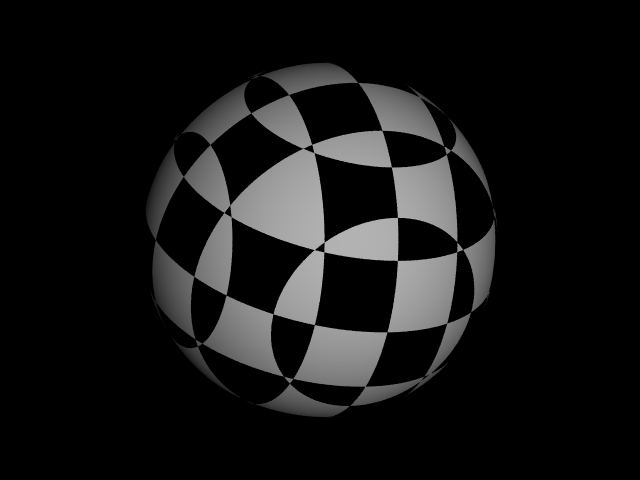
\includegraphics[width=170px]{left.png}
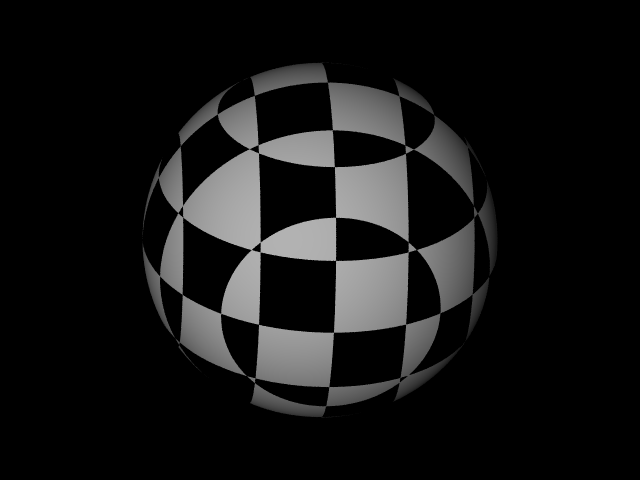
\includegraphics[width=170px]{right.png}
\end{center}
\caption{Image gauche et Image droite}
\end{figure}

\subsection{Matrice fondamentale}

Après la première étape, nous disposons de la matrice fondamentale suivante :
\begin{equation}
  \begin{bmatrix}
    -4.57132e-15 & -1.87385e+01 &  4.49723e+03\\
    -1.87384e+01 &  2.06585e-13 &  3.05726e+05\\
    4.49722e+03 & -2.93733e+05 & -2.87822e+06
  \end{bmatrix}
\end{equation}

\subsection{Coins et droites épipolaires}

Nous pouvons distinguer sur ces images les droites épipolaires (en vert) et les points correspondants aux coins trouvés par la méthode Shi-Tomasi (en rouge).\\ (Images disponibles en annexe)

\begin{figure}[h]
\begin{center}
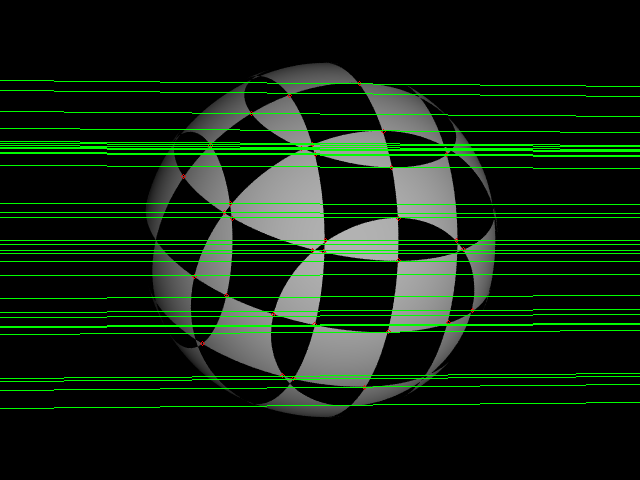
\includegraphics[width=170px]{left-result.png}
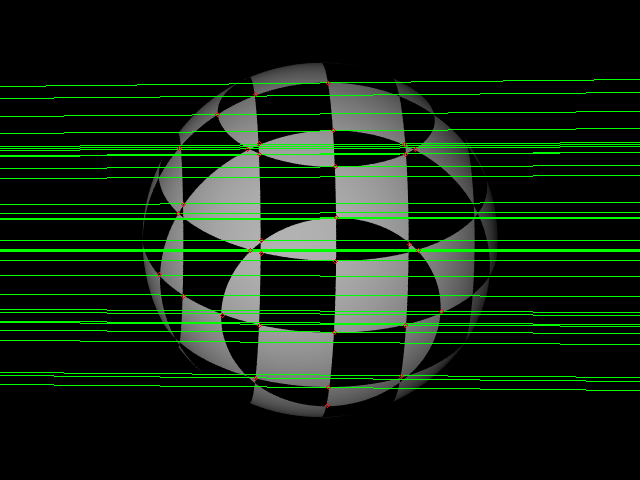
\includegraphics[width=170px]{right-result.png}
\end{center}
\caption{Coins et droites épipolaires}
\end{figure}

\subsection{Matrice des distances}

Après calcul des distances, nous sommes en présence d'une matrice de distances de 32x32 contenant ces informations :
\begin{equation}
\begin{bmatrix}
4.29133e-01 & 8.40214e+01 & 6.60562e+01 & 6.40529e+01 & ...\\
8.39824e+01 & 3.90121e-01 & 1.81575e+01 & 2.01317e+01 & ...\\
...
\end{bmatrix}
\end{equation}

\clearpage
%----------------------------------------------------------------------------------------

%----------------------------------------------------------------------------------------
%	CONCLUSION
%----------------------------------------------------------------------------------------

\section{Conclusion}

Nous avons constaté qu'un des problèmes de la photographie est qu'elle ne permet pas de conserver certaines informations, en particulier les informations sur la profondeur.\\

Nous avons donc choisi d'utiliser la méthode de la stéréoscopie, dont l'avantage est d'être peu complexe et facile à mettre en œuvre.\\

Après application de cette méthode, nous avons été en mesure de mettre en relations des points remarquables dans des projections d'une même scène, avec différents points de vue. Une fois les paires de points formées, nous avons pu reconstituer partiellement l'information de profondeur de la scène en 3D.\\

Cette méthode est cependant limitée par la qualité et la quantité des projections à disposition. De plus, nous ne pouvons pas reconstituer la totalité de la scène, car des objets pourront être cachés par d'autres objets.\\

Nous pouvons imaginer que cette méthode soit intéressante dans le cadre de la réalité virtuelle, afin de pouvoir récupérer les informations 3D d'une scène vue par l'utilisateur, les traiter, et pouvoir, entre autres, placer des objets ou des informations dans la scène afin de créer de la réalité augmentée.\\

\clearpage
%----------------------------------------------------------------------------------------

\section{Annexe}

\subsection{Résultats de la méthode Shi-Tomasi}
\begin{figure}[h]
\begin{center}
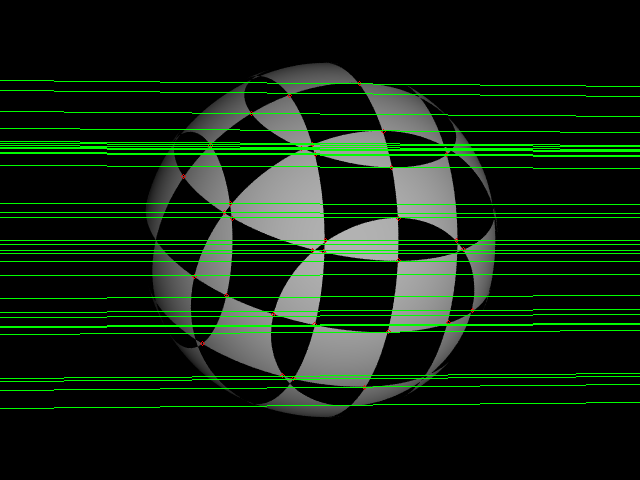
\includegraphics[width=450px]{left-result.png}
\end{center}
\caption{Coins et droites épipolaires - Image gauche}
\end{figure}

\begin{figure}[h]
\begin{center}
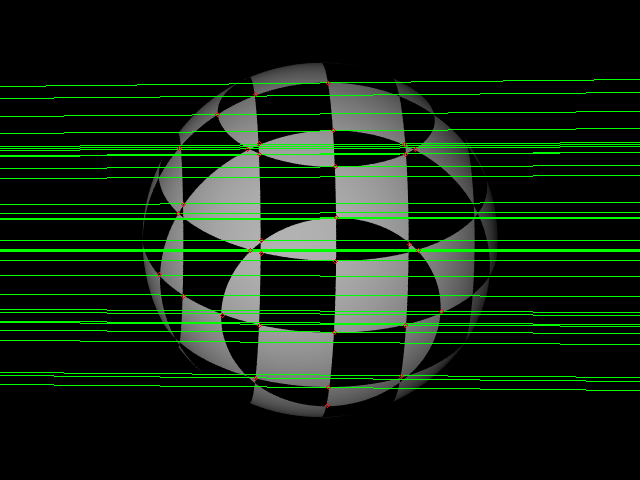
\includegraphics[width=450px]{right-result.png}
\end{center}
\caption{Coins et droites épipolaires - Image droite}
\end{figure}

\clearpage
\subsection{Fichier résultat après calcul des distances}

\lstinputlisting{resultats_distances.txt}


\end{document}
